% $Id: Michael.tex 11 2007-04-03 22:25:53Z jpeltier $

\documentclass{vgtc}                          % final (conference style)
%\documentclass[review]{vgtc}                 % review
%\documentclass[widereview]{vgtc}             % wide-spaced review
%\documentclass[preprint]{vgtc}               % preprint
%\documentclass[electronic]{vgtc}             % electronic version

%\documentclass{article}
\usepackage{ngerman}
\usepackage[T1]{fontenc}
\usepackage[utf8]{inputenc}

\usepackage[obeyspaces]{url}
\usepackage{hyperref}
\usepackage{subfigure}
\usepackage{amsmath}


\newcommand{\trajecmp}{\href{https://github.com/maiermic/trajecmp}{trajecmp}}
\newcommand{\BoostGeometry}{\href{http://www.boost.org/doc/libs/1_60_0/libs/geometry/doc/html/index.html}{Boost Geometry}}
\newcommand{\RxCpp}{\href{https://github.com/Reactive-Extensions/RxCpp}{RxCpp}}
\newcommand{\rangeLib}{\href{https://github.com/ericniebler/range-v3}{range-v3}}

\newcommand{\modifiedHausdorffDistFn}{modified Hausdorff distance function~\cite{modified_hausdorff}}



%%%%%%%%%%%%%%%%%%%%%%%
% syntax highlighting
%%%%%%%%%%%%%%%%%%%%%%%



\usepackage{color}
\usepackage[dvipsnames,table,xcdraw]{xcolor}
\usepackage{realboxes}
\usepackage{listings}
\definecolor{listinggray}{gray}{0.9}
\definecolor{lbcolor}{rgb}{0.9,0.9,0.9}
\definecolor{verylightgray}{rgb}{0.95,0.95,0.95}
\lstset{
backgroundcolor=\color{lbcolor},
tabsize=4,
%   rulecolor=,
language=[GNU]C++,
basicstyle=\scriptsize,
upquote=true,
aboveskip={1.5\baselineskip},
columns=fixed,
showstringspaces=false,
extendedchars=false,
breaklines=true,
prebreak = \raisebox{0ex}[0ex][0ex]{\ensuremath{\hookleftarrow}},
frame=single,
numbers=left,
showtabs=false,
showspaces=false,
showstringspaces=false,
identifierstyle=\ttfamily,
keywordstyle=\color[rgb]{0,0,1},
commentstyle=\color[rgb]{0.026,0.112,0.095},
stringstyle=\color[rgb]{0.627,0.126,0.941},
numberstyle=\color[rgb]{0.205, 0.142, 0.73},
%        \lstdefinestyle{C++}{language=C++,style=numbers}’.
}
\lstset{
basicstyle=\scriptsize,
backgroundcolor=\color{lbcolor},
tabsize=4,
language=C++,
captionpos=b,
tabsize=3,
frame=lines,
numbers=left,
numberstyle=\tiny,
numbersep=5pt,
breaklines=true,
showstringspaces=false,
basicstyle=\footnotesize,
%  identifierstyle=\color{YellowOrange},
keywordstyle=\color[rgb]{0,0,1},
commentstyle=\color{ForestGreen},
stringstyle=\color{red}
}

\newcommand{\inlineCpp}[1]{\Colorbox{verylightgray}{\lstinline[language=C++]$#1$}}

%% Uncomment one of the lines above depending on where your paper is
%% in the conference process. ``review'' and ``widereview'' are for review
%% submission, ``preprint'' is for pre-publication, and the final version
%% doesn't use a specific qualifier. Further, ``electronic'' includes
%% hyperreferences for more convenient online viewing.

%% Please use one of the ``review'' options in combination with the
%% assigned online id (see below) ONLY if your paper uses a double blind
%% review process. Some conferences, like IEEE Vis and InfoVis, have NOT
%% in the past.

%% Figures should be in CMYK or Grey scale format, otherwise, colour 
%% shifting may occur during the printing process.

%% These few lines make a distinction between latex and pdflatex calls and they
%% bring in essential packages for graphics and font handling.
%% Note that due to the \DeclareGraphicsExtensions{} call it is no longer necessary
%% to provide the the path and extension of a graphics file:
%% \includegraphics{diamondrule} is completely sufficient.
%%
\ifpdf%                                % if we use pdflatex
\pdfoutput=1\relax                   % create PDFs from pdfLaTeX
\pdfcompresslevel=9                  % PDF Compression
\pdfoptionpdfminorversion=7          % create PDF 1.7
\ExecuteOptions{pdftex}
\usepackage{graphicx}                % allow us to embed graphics files
\DeclareGraphicsExtensions{.pdf,.png,.jpg,.jpeg} % for pdflatex we expect .pdf, .png, or .jpg files
\else%                                 % else we use pure latex
\ExecuteOptions{dvips}
\usepackage{graphicx}                % allow us to embed graphics files
\DeclareGraphicsExtensions{.eps}     % for pure latex we expect eps files
\fi%

%% it is recomended to use ``\autoref{sec:bla}'' instead of ``Fig.~\ref{sec:bla}''
\graphicspath{{figures/}{pictures/}{images/}{./}} % where to search for the images

\usepackage{microtype}                 % use micro-typography (slightly more compact, better to read)
\PassOptionsToPackage{warn}{textcomp}  % to address font issues with \textrightarrow
\usepackage{textcomp}                  % use better special symbols
\usepackage{mathptmx}                  % use matching math font
\usepackage{times}                     % we use Times as the main font
\renewcommand*\ttdefault{txtt}         % a nicer typewriter font
\usepackage{cite}                      % needed to automatically sort the references
\usepackage{tabu}                      % only used for the table example
\usepackage{booktabs}                  % only used for the table example
\usepackage{listings}
%% We encourage the use of mathptmx for consistent usage of times font
%% throughout the proceedings. However, if you encounter conflicts
%% with other math-related packages, you may want to disable it.


%% If you are submitting a paper to a conference for review with a double
%% blind reviewing process, please replace the value ``0'' below with your
%% OnlineID. Otherwise, you may safely leave it at ``0''.
\onlineid{0}

%% declare the category of your paper, only shown in review mode
\vgtccategory{Research}

%% allow for this line if you want the electronic option to work properly
\vgtcinsertpkg

%% In preprint mode you may define your own headline.
%\preprinttext{To appear in an IEEE VGTC sponsored conference.}

%% Paper title.

\title{MagicVR - Gesture Recognition}

%% This is how authors are specified in the conference style

%% Author and Affiliation (single author).
%%\author{Roy G. Biv\thanks{e-mail: roy.g.biv@aol.com}}
%%\affiliation{\scriptsize Allied Widgets Research}

%% Author and Affiliation (multiple authors with single affiliations).
%%\author{Roy G. Biv\thanks{e-mail: roy.g.biv@aol.com} %
%%\and Ed Grimley\thanks{e-mail:ed.grimley@aol.com} %
%%\and Martha Stewart\thanks{e-mail:martha.stewart@marthastewart.com}}
%%\affiliation{\scriptsize Martha Stewart Enterprises \\ Microsoft Research}

%% Author and Affiliation (multiple authors with multiple affiliations)
\author{Jerome D. Pönisch\thanks{e-mail: jerome.poenisch@campus.lmu.de}\\ %
\scriptsize 3D Models and Effects %
\and Michael Maier\thanks{e-mail: maier.michael@campus.lmu.de}\\ %
\scriptsize Gesture Recognition}

%% A teaser figure can be included as follows, but is not recommended since
%% the space is now taken up by a full width abstract.
%\teaser{
%  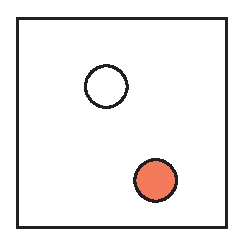
\includegraphics[width=1.5in]{sample.eps}
%  \caption{Lookit! Lookit!}
%}

%% Abstract section.
\abstract{This documentation is about MagicVR - a virtual reality application developed in OpenSG for the LRZ V2C in Garching supporting 3D-Gesture-Recognition and Lerp-Animations.
} % end of abstract

%% ACM Computing Classification System (CCS). 
%% See <http://www.acm.org/about/class> for details.
%% We recommend the 2012 system <http://www.acm.org/about/class/class/2012>
%% For the 2012 system use the ``\CCScatTwelve'' which command takes four arguments.
%% The 1998 system <http://www.acm.org/about/class/class/2012> is still possible
%% For the 1998 system use the ``\CCScat'' which command takes four arguments.
%% In both cases the last two arguments (1998) or last three (2012) can be empty.

\CCScatlist{
\CCScatTwelve{V2C}{Virtual Reality}{OpenSG}{Treemaps}{}
}

%\CCScatlist{
%\CCScat{H.5.2}{User Interfaces}{User Interfaces}{Graphical user interfaces (GUI)}{};
%\CCScat{H.5.m}{Information Interfaces and Presentation}{Miscellaneous}{}{}
%}

%% Copyright space is enabled by default as required by guidelines.
%% It is disabled by the 'review' option or via the following command:
% \nocopyrightspace

%%%%%%%%%%%%%%%%%%%%%%%%%%%%%%%%%%%%%%%%%%%%%%%%%%%%%%%%%%%%%%%%
%%%%%%%%%%%%%%%%%%%%%% START OF THE PAPER %%%%%%%%%%%%%%%%%%%%%%
%%%%%%%%%%%%%%%%%%%%%%%%%%%%%%%%%%%%%%%%%%%%%%%%%%%%%%%%%%%%%%%%%

\lstset{
breaklines=true,
tabsize=2,
}


\begin{document}

    %% The ``\maketitle'' command must be the first command after the
    %% ``\begin{document}'' command. It prepares and prints the title block.

    %% the only exception to this rule is the \firstsection command
    \firstsection{Introduction}

    \maketitle

    %% \section{Introduction} %for journal use above \firstsection{..} instead
    In this documentation the concept and implementation of MagicVR gestures will be
explained. MagicVR is a virtual reality application which was developed in C++
and OpenSG in order to run in the V2C mixed reality cave of the LRZ in Garching,
Munich. It\rq{}s main feature is a 3D-Gesture-Recognition opening a whole world
of interaction possibilities using only the wand (or any tracker) in a 3D
tracking system.

    \section{Concept}

MagicVR was developed in a cooperation between Jerome Pönisch and Michael Maier. This paper will be focused on the 3D Art and FractTime-Animation effects done by Jerome Pönisch while Michaels\rq{}s paper will be focused on the 3D-Gesture-Recognition.
This section shall introduce in the general concept of MagicVR and the effects and animation part.

\subsection{The idea behind MagicVR}

The main idea of MagicVR is introducing the 3D-Gesture-Recognition module in a playful environment using important features of a virtual environment. A user/player should be animated to use 3D-Gestures as interesting interaction technique rather than pushing buttons. The virtual environment should help to gain the user/player\rq{}s interest and make him feel comfortable while experiencing the mixed reality world. As User-Feedback it was decided to focus on animations and movements within the scene.

\subsection{FractTime-Animations}

In order to make movements easier to implement and control a framework was implemented based on the idea of Vector Lerp, FractTime and Coroutines from Unity and C\#.
\begin{description}
 \item{\textbf{Lerp}} is a commonly used short term standing for \lq\lq{}linear interpolation\rq\rq{}. The concept of a Vector.Lerp in Unity and C\# takes an original vector and a target vector and makes a linear interpolation between those two vectors using an interpolation factor from 0 to 1.
 
 \item{\textbf{FracTime}} is used as the interpolation factor in our framework. It devides the already animated time by the target duration of the animation providing a factor between 0 and 1.
 
 \item{\textbf{Coroutines}} are used in Unity to run multible routines at the same time which makes it easier to control them individually. The difference to c++ is, that multithreading is more trivial in C\#.
 \end{description}
 
 Those two concepts were used in combination to write our own FractTime-Animations framework.\\
 
 \subsection{Advantages of FracTime Animations}
 The advantages of using our animation framework are among others:
 \begin{description}
 \item{\textbf{Trustability}} Destination and Target values of vectors, colors etc. are clear defined and thereby no \lq\lq{}surprises will happen during animations\rq\rq{}
 \item{\textbf{Controlability}} Since all animations are placed and controlled in one main container and subcontainers, each animation can be started and stopped individually.
 \item{\textbf{FPS-Stability}} Since the animations are based on the FracTime, which is based on the delta time between frames, and not e.g. the translation distance animations will allways take the same time independent of the FPS given by the render system.
 \end{description}

    \section{Implementation}

The project is implemented in C++ using the libraries \BoostGeometry, \RxCpp, \rangeLib and \trajecmp.
The library \trajecmp is written by the author Michael Maier to detect gestures.
The process shown in~\autoref{fig:system-diagram} is implemented like this:

\begin{lstlisting}
const auto result_stream =
    compare(preprocess(input_stream),
            preprocess(pattern_stream));

result_stream.subscribe([](auto result) {
    // process result
});
\end{lstlisting}

\noindent
\inlineCpp{input\_stream} and \inlineCpp{pattern\_stream} are streams of trajectories.
Every time a input trajectory is emitted on \inlineCpp{input\_stream} it is preprocessed and compared with the (latest) preprocessed pattern trajectory of \inlineCpp{pattern\_stream}.
Usually, \inlineCpp{pattern\_stream} contains only one (static pattern) trajectory.
However, a pattern trajectory might be dynamically created.
For example, you could use another input trajectory as a pattern.\\

\noindent
You can compare the input trajectory with multiple patterns like this:

\begin{lstlisting}
const auto preprocessed_input_stream =
    preprocess(input_stream);

const auto result_1_stream =
    compare(preprocessed_input_stream,
            preprocess(pattern_1_stream));

const auto result_2_stream =
    compare(preprocessed_input_stream,
            preprocess(pattern_2_stream));

result_1_stream.subscribe([](auto result) {
    // process result
});

result_2_stream.subscribe([](auto result) {
    // process result
});
\end{lstlisting}

\noindent
All gestures of the project are implemented in the class \path{sources/magicvr/MagicTricks.cpp}.
Apart from the preprocessing steps shown in~\autoref{fig:preprocessing-steps} it contains a rotation transformation around the axis pointing upwards in the cave.
The event subscription is done in \path{sources/magicvr/AppController.cpp} and \path{sources/magicvr/AppControllerWithWandSupport.cpp}.

    \section{Gestures}
In this section the gestures are described.
The effect of each gesture is described in Jerome\rq{}s documentation.

\subsection{Fire}
The fire gesture (see~\autoref{fig:fire-gesture}) is a flame symbol drawn from left to right.
It is defined by this trajectory:

\begin{lstlisting}
Trajectory{
    {0,  0, 0},
    {-1, 3, 0},
    {1,  2, 0},
    {2,  5, 0},
    {2,  5, 0},
    {3,  2, 0},
    {5,  3, 0},
    {4,  0, 0},
}
\end{lstlisting}

\begin{figure}[!ht]
    \includegraphics[width=0.4\textwidth]{pictures/fire-gesture.jpg}
    \caption{Fire gesture}
    \label{fig:fire-gesture}
\end{figure}


\subsection{Water}
The water gesture (see~\autoref{fig:water-gesture}) is a wave symbol drawn from left to right.
It is defined by this bezier curve:

\begin{lstlisting}
const BezierCurve<> waterBezier{
    {0,    0,  0},
    {1.5f, 3,  0},
    {1.5f, -2, 0},
    {3,    1,  0},
};
\end{lstlisting}

\begin{figure}[!ht]
    \includegraphics[width=0.4\textwidth]{pictures/water-gesture.jpg}
    \caption{Water gesture}
    \label{fig:water-gesture}
\end{figure}


\subsection{Lightning}
The lightning gesture (see~\autoref{fig:lightning-gesture}) is a lightning symbol drawn from top to bottom.
It is defined by this trajectory:

\begin{lstlisting}
Trajectory{
    {1, 2, 0},
    {0, 1, 0},
    {1, 1, 0},
    {0, 0, 0},
}
\end{lstlisting}

\begin{figure}[!ht]
    \includegraphics[width=0.4\textwidth]{pictures/lightning-gesture.jpg}
    \caption{Lightning gesture}
    \label{fig:lightning-gesture}
\end{figure}


\subsection{Wind}
The wind gesture (see~\autoref{fig:wind-gesture}) is a spiral drawn from the inside to the outside.
The trajectory is calculated in the method \inlineCpp{sample} of the class \path{sources/magicvr/Spiral.cpp}.

\begin{figure}[!ht]
    \includegraphics[width=0.4\textwidth]{pictures/wind-gesture.jpg}
    \caption{Wind gesture}
    \label{fig:wind-gesture}
\end{figure}


\subsection{Circle}\label{subsec:circle}
The circle gesture (see~\autoref{fig:circle-gesture}) is a single circle drawn from the left side of the center to the top.
The trajectory is calculated in the method \inlineCpp{sample} of the class \path{sources/magicvr/ranges/view/Circle.cpp}.

\begin{lstlisting}
Circle(1).sample(0, 360, 10)
\end{lstlisting}

\begin{figure}[!ht]
    \centering
    
\includegraphics[width=0.15\textwidth]{pictures/circle-gesture.png}
    \caption{Circle gesture}
    \label{fig:circle-gesture}
\end{figure}


\subsection{Multiplication}
The multiplication gesture is a~\nameref{subsec:circle} gesture with two circumnavigations.

\begin{lstlisting}
Circle(1).sample(0, 720, 10)
\end{lstlisting}


\subsection{Shoot}
The shoot gesture (see~\autoref{fig:shoot-gesture}) is a quarter segment of a circle drawn from above with a circumnavigation direction to the right (in the style of a whip movement).

\begin{lstlisting}
const BezierCurve<> quaterCircleFromAbove{
        {0, 1, 0},
        {1, 1, 0},
        {1, 0, 0},
        {1, 0, 0},
};
\end{lstlisting}

\begin{figure}[!ht]
    \centering
    
\includegraphics[width=0.15\textwidth]{pictures/shoot-gesture.png}
    \caption{Shoot gesture}
    \label{fig:shoot-gesture}
\end{figure}

    \section{Outlook}

The implemented animation framework makes it easy to implement further animation types and more complex movements while they stay very control- and adjustable. There are multiple further ways how and where this animation framework could be applied e.g. animating not only Vectors but also materials, colors, transparency etc.\\

Since there wasn\rq{}t enough time to finish all our ideas, the interactions for lightning and wind bubbles was not completely implemented. Hitting the lantern with lightning bubbles should have lit up the scene bit by bit as if the light was trapped inside the lantern. The wind gesture should have activated a kind of manipulation mode in combination with a second gesture setting a direction. With this combination it should have been possible to move the lantern around in the scene in order to light up different parts of the scene.\\

Also because of the lack of time there was no opportunity to implement a better user guidance. Our idea would have been to implement a little fairy which gives hints about interaction possibilities and demonstrates according gestures by flying them in front of the user.



    %\bibliographystyle{abbrv}
    \bibliographystyle{abbrv-doi}
    %\bibliographystyle{abbrv-doi-narrow}
    %\bibliographystyle{abbrv-doi-hyperref}
    %\bibliographystyle{abbrv-doi-hyperref-narrow}

    \bibliography{Michael}
\end{document}
